\usetikzlibrary{arrows.meta,calc,shapes}
\providecommand{\computer}{%
    
\includegraphics[width=1cm,alt={computer}]{../common/Noun_project_216.pdf}
}
\providecommand{\switch}{%
    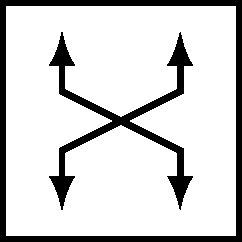
\includegraphics[width=0.9cm,alt={switch}]{../common/fig-switch.pdf}
}
\providecommand{\router}{%
    
\includegraphics[width=0.9cm,alt={router}]{../common/fig-router.pdf}
}


\begin{frame}\frametitle{networks / hosts aka end systems}
\myalttextD{%
\begin{tikzpicture}
\tikzset{
    connect/.style={draw,very thick,Latex-Latex},
    computer/.style={inner sep=0mm,outer sep=0mm,beameralt=<4>{label={[font=\small,label distance=0mm,text=red]south:`host'}},execute at begin node={\computer}},
}
\node[
      cloud,draw,very thick,aspect=2,
      minimum width=4cm,minimum height=3cm,
      beameralt=<2-3>{draw=red,fill=red!10,label={[text=red]center:`network'}},
     ] (net-cloud) at (0,0) {};
\foreach \x/\d in {0/5cm,45/4cm,90/3cm,135/4cm,180/5cm,225/4cm,270/3cm,315/4cm} {
    \node[computer] (c-\x) at (\x:\d) {};
    \draw[connect] (net-cloud) -- (c-\x);
}
\coordinate (box loc) at (4cm, 3.5cm);
\tikzset{
    explain box/.style={
        overlay,draw=red, align=left, very thick, anchor=north west
    },
}
\begin{visibleenv}<2>
\node[explain box] at (box loc) {
    \textit{networks} connect \\
    computers 
};
\end{visibleenv}
\begin{visibleenv}<3>
\node[explain box] at (box loc) {
    `cloud' represents \\
    any network \\
    (whether local or not) \\
    \small iconography predates \\
    \small `cloud computing'
};
\end{visibleenv}
\begin{visibleenv}<4>
\node[explain box] at (box loc) {
    computers on edge \\
    of network called \\
    \textit{hosts} or \textit{end systems} \\
    \small (even if also `servers')
};
\end{visibleenv}
\end{tikzpicture}
}{
Picture showing computers connected via lines with arrowheads on both ends to a cloud.
}{
Same diagram as previous slide. The cloud is labeled as a `network' and a box reads ``networks connect computers''.
}{
Same diagram as previous slide. The cloud is labeled as a `network' and a box reads ``cloud represents any network (whether local or not). Iconography predates cloud computing.''
}{
Same diagram as previous slide. The computers are labeled `hosts' and a box reads ``computers on edge of network called hosts or end systems (even if also `severs').''
}
\end{frame}

\begin{frame}\frametitle{direct connections?}
\myalttext{%
\begin{tikzpicture}
\tikzset{
    connect/.style={draw,very thick,Latex-Latex},
    computer/.style={inner sep=0mm,outer sep=0mm,execute at begin node={\computer}},
}
\foreach \x/\d in {0/5cm,45/4cm,90/3cm,135/4cm,180/5cm,225/4cm,270/3cm,315/4cm} {
    \node[computer] (c-\x) at (\x:\d) {};
    \foreach \y in {0,45,90,135,180,225,270,315} {
        \ifnum \x = \y
            \relax
        \else
            \draw[connect] (c-\x) -- (c-\y);
        \fi
    }
}
\end{tikzpicture}
}{%
Picture showing 8 computers connected to each other via 56 lines (one for each pair of computers).
}
\end{frame}

\begin{frame}\frametitle{shared medium: radio?}
\myalttext{%
\begin{tikzpicture}
\tikzset{
    connect/.style={draw,very thick,Latex-Latex},
    computer/.style={inner sep=0mm,outer sep=0mm,execute at begin node={\computer}},
}
\foreach \x/\d in {0/5cm,45/4cm,90/3cm,135/4cm,180/5cm,225/4cm,270/3cm,315/4cm} {
    \node[computer] (c-\x) at (\x:\d) {};
%    %\begin{visibleenv}<2->
    \pgfmathsetmacro\oppX{\x+180}
    \path (c-\x.\oppX) -- ++(\oppX:0.1) coordinate (c-\x-wifi);
    \foreach \y in {0.2,0.35,0.5} {
        \draw[ultra thick] (c-\x-wifi) ++ (\oppX-50:\y) arc (\oppX-50:\oppX+50:\y);
    }
%    %\end{visibleenv}
}
\end{tikzpicture}
}{%
Picture showing the same 8 computers with wifi-like symbols indicating they communicate via radio.%
}
\end{frame}

\begin{frame}\frametitle{shared medium: wires}
\myalttextC{%
\begin{tikzpicture}
\tikzset{
    connect/.style={draw,very thick,arrows={Latex-Circle[width=0.3cm,length=0.3cm]},
        beameralt=<2>{arrows={Latex-Circle[width=0.3cm,length=0.3cm,red]}}},
    computer/.style={inner sep=0mm,outer sep=0mm,execute at begin node={\computer}},
}
\draw[line width=1mm] (-5,-1.5) coordinate (wire start) -- (5, 1.5) coordinate (wire end);
\foreach \x/\d in {0/5cm,45/4cm,90/3cm,135/4cm,180/5cm,225/4cm,270/3cm,315/4cm} {
    \node[computer] (c-\x) at (\x:\d) {};
    \coordinate (connect-\x) at ($(wire start)!(c-\x.center)!(wire end)$);
    \draw[connect] (c-\x) -- (connect-\x) -- ([turn]0:.1cm);
}
\begin{visibleenv}<2-3>
\node[anchor=north west,fill=white,draw=black,thick,label={[font=\tiny]south:Ali at gwc.org.uk / Alistair1978 via Wikimedia commons / CC-BY-SA 2.5}] 
    (thicknet) at (4, 3.5) {
    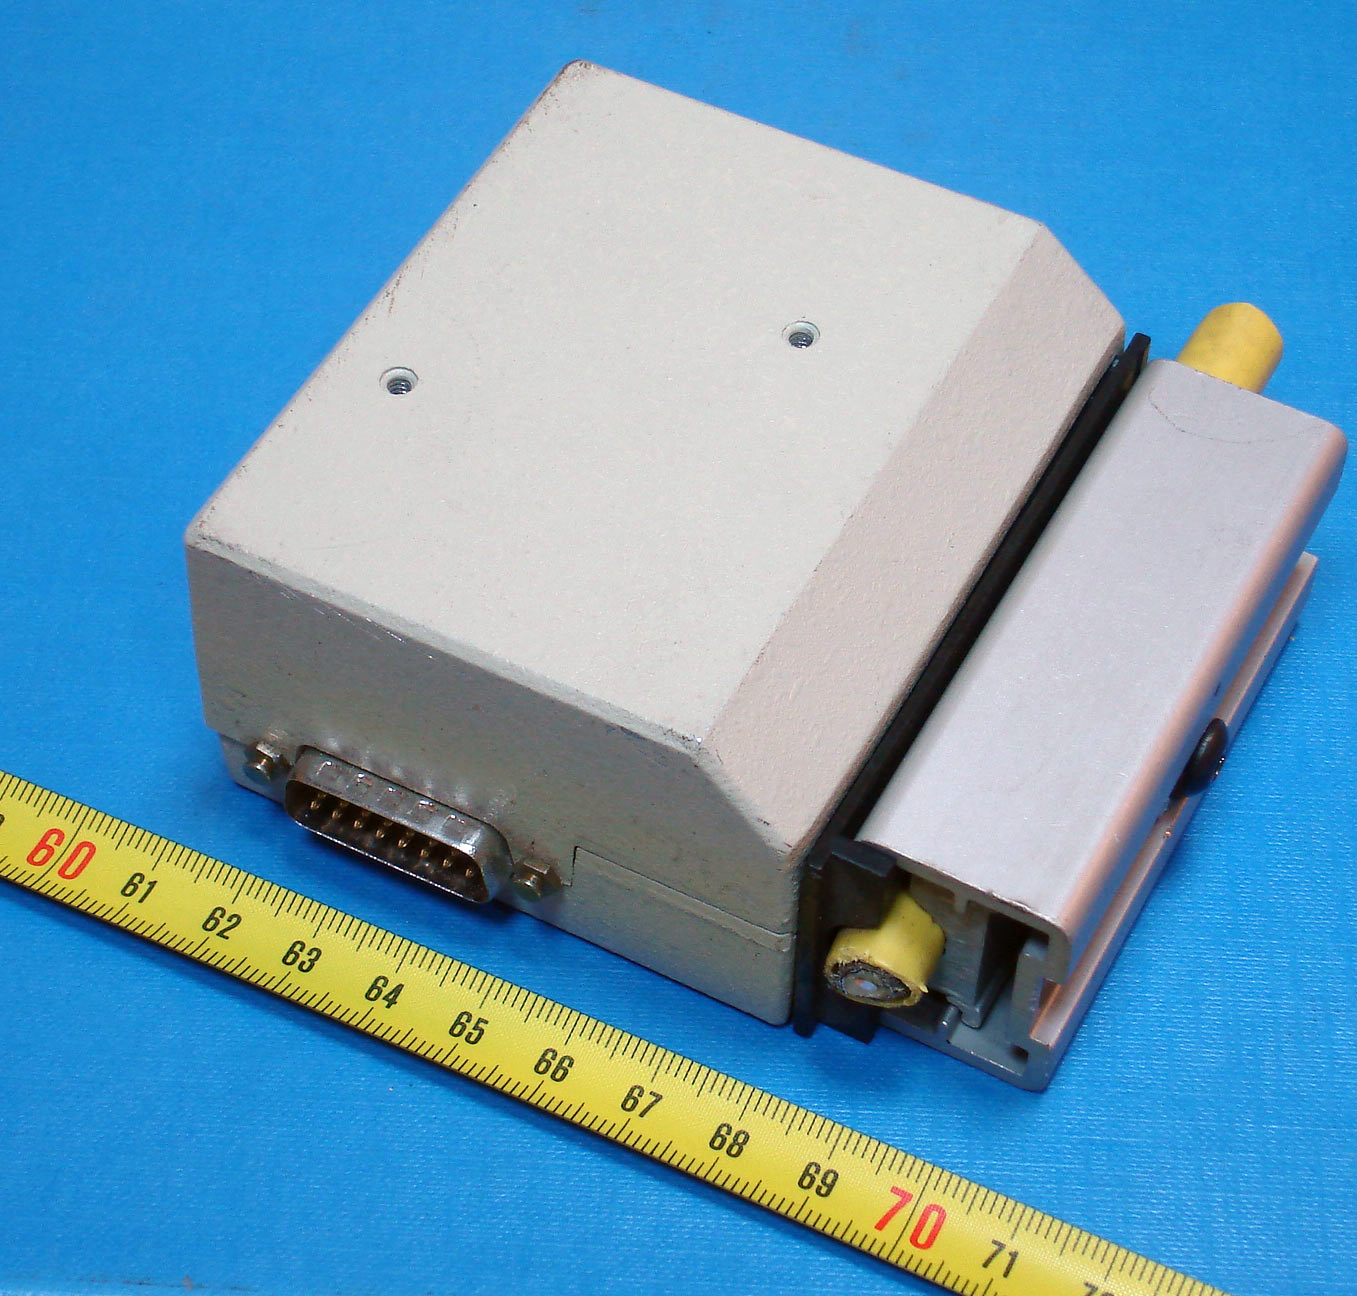
\includegraphics[width=4cm]{../intro/ThicknetTransceiver.jpeg}
};
\end{visibleenv}
\begin{visibleenv}<3>
\node[fill=white,draw=black,thick,anchor=north west] at ([yshift=-0.75cm]thicknet.south west) {
    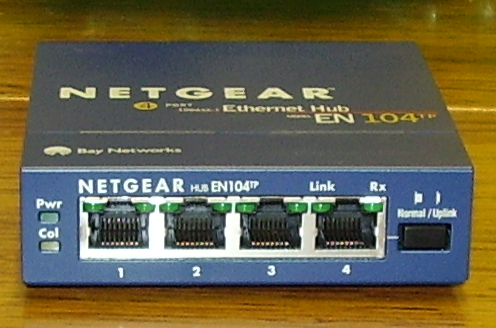
\includegraphics[width=4cm]{../intro/4_port_netgear_ethernet_hub}
};
% FIXME: also fiber splitter
\end{visibleenv}
\end{tikzpicture}
}{
Picture showing 8 computers connected via vertical lines to a single horizontal line representing a wire.
}{
Same picture as before with the connection between the vertical lines and horizontal lines highlighted, and a picture of a Thicknet transciever, a device
that screws into coax cable to provide an electrical connection.
}{
Same picture as before with the addition of a picture of a 4-port Ethernet hub --- a Netgear-branded box with four RJ-45 ports.
}
\end{frame}

\begin{frame}\frametitle{switches / nodes / links}
\myalttext{
\begin{tikzpicture}
\tikzset{
    computer/.style={inner sep=0mm,outer sep=0mm,execute at begin node={\computer},beameralt=<3>{fill=red!10}},
    switch/.style={inner sep=0mm,outer sep=0mm,execute at begin node={\switch},
                   beameralt=<2>{
                       fill=red!10,
                        label={[font=\small,label distance=0mm,text=red]south:`switch'}
                   },
                   beameralt=<3>{fill=red!10}},
    connect/.style={draw,very thick,Latex-Latex,beameralt=<4>{red}},
    connect big/.style={draw,ultra thick,Latex-Latex,beameralt=<4>{red}},
}
\node[
      cloud,draw,opacity=0.25,very thick,aspect=2,
      minimum width=7cm,minimum height=4cm,
     ] (net-cloud) at (0,0) {};
\foreach \x/\d in {0/5cm,45/4cm,90/3cm,135/4cm,180/5cm,225/4cm,270/3cm,315/4cm} {
    \node[computer] (c-\x) at (\x:\d) {};
}
\node[switch] (s1) at (2,-0.5) {};
\node[switch] (s2) at (-1,0.5) {};
\node[switch] (s3) at (0,-1) {};
\draw[connect] (c-0) -- (s1);
\draw[connect] (c-45) -- (s1);
\draw[connect] (c-315) -- (s1);
\draw[connect] (c-90) -- (s2);
\draw[connect] (c-135) -- (s2);
\draw[connect] (c-180) -- (s2);
\draw[connect] (c-225) -- (s3);
\draw[connect] (c-270) -- (s3);
\draw[connect big] (s1) -- (s2);
\draw[connect big] (s1) -- (s3);
\coordinate (box loc) at (4cm, 4.5cm);
\begin{visibleenv}<2>
\node[overlay,draw=red, align=left, very thick, anchor=north west] at (box loc) {
    hosts directly connected to \\
    \textit{\myemph{switches}} \\
    that implement network \\
    ~ \\
    (more efficiently than \\
    shared medium)
};
\end{visibleenv}
\begin{visibleenv}<3>
\node[overlay,draw=red, align=left, very thick, anchor=north west] at (box loc) {
    machines on network \\
    (hosts, switches, \ldots) \\
    called \textit{\myemph{nodes}}
};
\end{visibleenv}
\begin{visibleenv}<4>
\node[overlay,draw=red, align=left, very thick, anchor=north west] at (box loc) {
    nodes connected by \\
   \textit{\myemph{links}} \\
    ~ \\
    (implemented by wires \\
    or radio or \ldots)
};
\end{visibleenv}
\end{tikzpicture}
}{
Diagram of computers connected by a network. Lines with arrowheads
at both ends extend from the computers to a number of boxes (with
a design of crossing lines with arrowheads). Later frames
repeat the diagram and indicate the boxes are called `switches';
every participant (computers and switches) are called `nodes';
and the lines connecting them are called `links' (regardless
of whether implemented with wires or radio or whatever).
}
\end{frame}

% FIXME: picture of physical switch

\begin{frame}\frametitle{routers / internetwork}
\myalttext{%
\begin{tikzpicture}
\tikzset{
    computer/.style={inner sep=0mm,outer sep=0mm,execute at begin node={\computer}},
    switch/.style={inner sep=0mm,outer sep=0mm,execute at begin node={\switch}},
    router/.style={inner sep=0mm,outer sep=0mm,execute at begin node={\router},circle,
        beameralt=<2>{fill=red!10}},
    connect/.style={draw,very thick,Latex-Latex},
    connect big/.style={draw,ultra thick,Latex-Latex},
}
\node[
      cloud,draw,opacity=0.25,very thick,aspect=2,
      minimum width=3cm,minimum height=2cm,
     ] (net-1) at (-1,1) {};
\node[
      cloud,draw,opacity=0.25,very thick,aspect=2,
      minimum width=3cm,minimum height=2cm,
     ] (net-2) at (3,0) {};
\node[
      cloud,draw,opacity=0.25,very thick,aspect=2,
      minimum width=3cm,minimum height=2cm,
     ] (net-3) at (-2,-4) {};
\node[
      cloud,draw,opacity=0.25,very thick,aspect=2,
      minimum width=3cm,minimum height=2cm,
     ] (net-4) at (2,-3) {};
%
\node[
      cloud,draw,opacity=0.25,very thick,aspect=2,
      minimum width=3cm,minimum height=2cm,
     ] (net-5) at (6,-4) {};
% FIXME: routers
\node[router] (r1) at (-2, -1.5) {};
\draw[connect big] (r1) -- (net-1);
\draw[connect big] (r1) -- (net-2);
\draw[connect big] (r1) -- (net-3);
\node[router] (r2) at (5, -2) {};
\draw[connect big] (r2) -- (net-4);
\draw[connect big] (r2) -- (net-5);
\draw[connect big] (r2) -- (net-2);
\node[router] (r3) at (3, -5) {};
\draw[connect big] (r3) -- (net-3);
\draw[connect big] (r3) -- (net-5);
\coordinate (box loc) at (6, 2);
\tikzset{
    explain box/.style={
        overlay,draw=red, align=left, very thick, anchor=north west
    },
}
\begin{visibleenv}<2>
\node[explain box] at (box loc) {
    \textit{\myemph{routers}} or \textit{\myemph{gateways}} \\
    connect networks
};
\end{visibleenv}
\begin{visibleenv}<3>
\node[explain box] at (box loc) {
    connected networks \\
    form \textit{\myemph{internetwork}}
    ~ \\
    (example: the Internet)
};
\end{visibleenv}
\end{tikzpicture}
}{Diagram of clouds representing networks connected via bidirectional
links to circles with two diagonal arrowheads representing `routers' 
or `gateways' that connect network.
}
\end{frame}
